\graphicspath{{images_low_res/}}

\section{Background of Research}
\label{sec:background}

\subsection{A Comparison of Methods for Screening Strain Fitness }

QFA and SGA are methods for high-throughput fitness screening using cultures grown on
solid agar \citep{Baryshnikova2010sga,Banks2012}. SGA uses a single measurement of culture
size, taken at some midpoint in the growth curve, as a surrogate for growth rate
\citep{Baryshnikova2010sga}. QFA collects more information about growth by taking images
of plates at points throughout the growth curve. QFA can be performed using either the
pinned cultures used in SGA or dilute liquid cultures (``spots'') of lower initial cell
density. Although pinned QFA allows for more cultures per plate (1536 vs 384 in spotted),
spotted QFA allows for more accurate fitting of growth models as growth curves are more
complete (see Figure~\ref{fig:qfa_and_sga_growth_curves}) \citep{Lawless2010}. Comparison
of spotted and pinned QFA cultures in Figure~\ref{fig:qfa_and_sga_growth_curves}c shows
how spotted cultures are composed of many individual colonies which increase in size and
thickness, whereas pinned cultures are composed of a single uniform colony which grows
radially. The number of individual colonies in a spotted culture is high enough that lag
and other stochastic effects should average out.

Colonyzer \citep{Lawless2010}, a QFA tool for automatic capture of growth curves, from
images of both spotted and pinned plates, uses integrated optical density (IOD) as a proxy
for cell density. Figure~\ref{fig:qfa_curves} \citep{Banks2012}, shows an example of 308
growth curves from a spotted QFA plate captured by Colonyzer and assembled by the QFA R
package \citep{qfa2016}. In SGA, culture area, rather than IOD, is used as a proxy for
culture density \citep{Baryshnikova2010sga}. \citet{Lawless2010} find that direct area
measurements are more noisy than IOD measurements and provide a worse fit to the logistic
model. To prevent bias in comparison of experimental designs, we will use Colonyzer to
generate more accurate IOD measurements from spotted and pinned QFA images.

Fitness screening can also be performed using independent liquid cultures which are not susceptible to
competition or signalling effects \citep{Jasnos2007}. However, this approach has lower throughput.

\end{multicols}
\graphicspath{{images_low_res/}}
\begin{Figure}
  \centering
  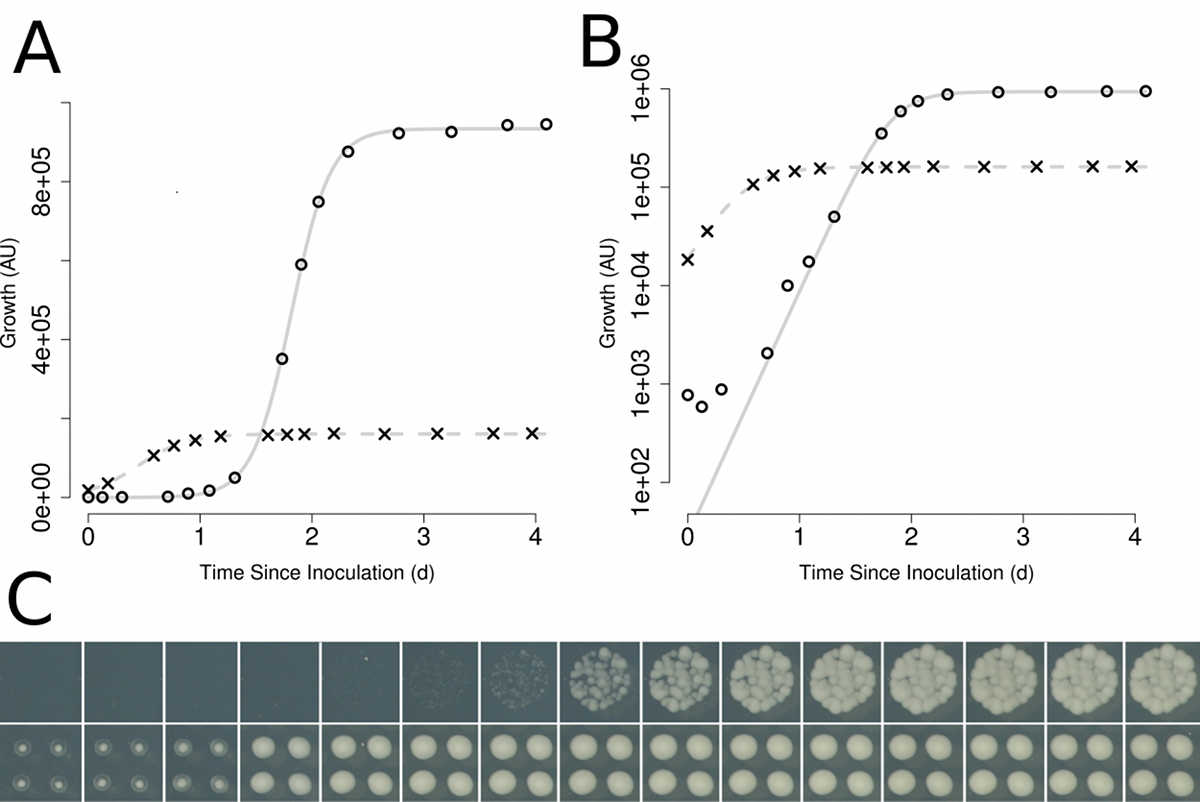
\includegraphics[width=\linewidth]{pin_v_spot_growth}
  \captionof{figure}{Fits of the logistic growth model, to cell density observations of
    yeast growing on solid agar, for spotted (circles) and pinned (crosses) QFA
    cultures. In A) cell density is plotted on a linear scale. In B) cell density is
    plotted on a logarithmic scale. C) shows images of the spotted and pinned cultures
    corresponding to the data in A) \& B) \citep{Lawless2010}.}
  \label{fig:qfa_and_sga_growth_curves}
\end{Figure}
\begin{multicols}{2}


\end{multicols}
\graphicspath{{images_low_res/}}
\begin{Figure}
  \centering
  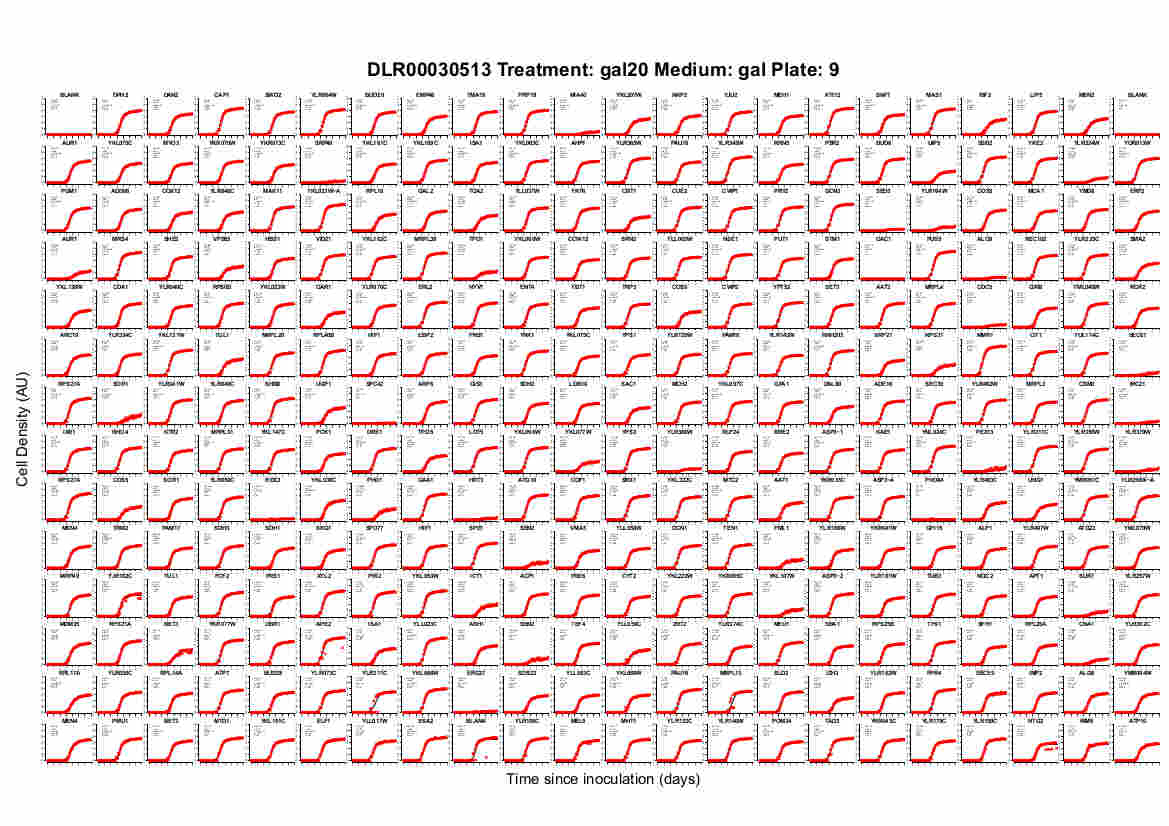
\includegraphics[width=\linewidth]{qfa_growth_array}
  \captionof{figure}{308 growth curves from a spotted QFA plate captured by Colonyzer \citep{Lawless2010} and assembled
    by the QFA R package \citep{qfa2016} \citep{Banks2012}.}
  \label{fig:qfa_curves}
\end{Figure}
\begin{multicols}{2}


\subsection{Competition and Signalling}

At the beginning of QFA, nutrients are distributed uniformly throughout the
agar. During incubation, cultures grow, consuming nutrients and creating gradients in
nutrient density. A QFA plate taken partway through incubation can be
seen in Figure~\ref{fig:15_spots}. As some cultures grow much faster than their
neighbours, using more nutrients, we believe that diffusion of nutrients along gradients
between cultures might cause a significant competition effect. Growth of yeast cultures
may also be affected by signal molecules produced by cells, which diffuse through the
agar or travel across its surface. Candidates are ethanol \citep{fujita2006}, a poison
produced by fermentation, and ammonia which is involved in regulatory response
to changes in cell density (quorum sensing) \citep{sprague2006,honigberg2011}.

\begin{Figure}
  \centering
  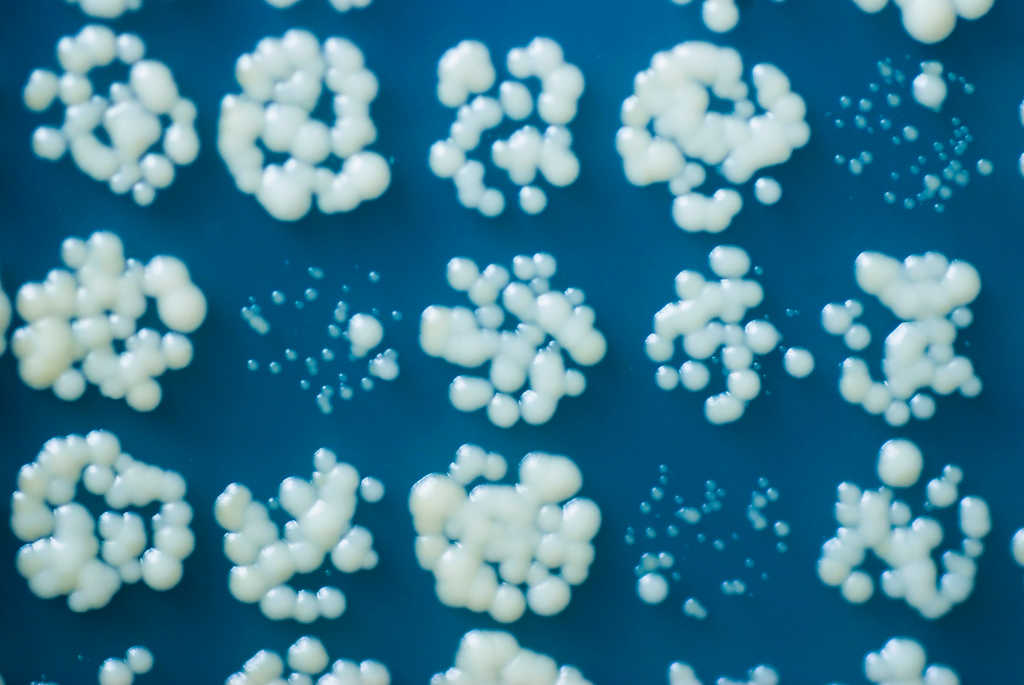
\includegraphics[width=\linewidth]{5658435523_c2e43729f1_b}
  \captionof{figure}{An image of 15 cultures on a section of solid agar from a QFA
    procedure. \citep{Lawless2010} https://github.com/CnrLwlss/Colonyzer}
  \label{fig:15_spots}
\end{Figure}

\subsection{Modelling Approaches}

\subsubsection{Mass Action Kinetics}
Chemical reactions are commonly modelled using mass action kinetics, where the rate of a
reaction in a well stirred mixture is proportional to the product of the concentrations of
the reactants. This accurately reflects the probabilistic nature of reactions in the gas
phase, which arise from collisions between reactants travelling at high velocity in random
directions. If species numbers are large enough, reactions can be modelled continuously
and deterministicly using ordinary differential equations (ODEs). Microbial population
growth, with cell division dependent on nutrient availability, can also be modelled using
mass action kinetics. We can use the following reaction equation for a culture \(i\)
growing on the agar,
\begin{subequations}
  \label{eq:9}
  \begin{align}
    &N + C \xrightarrow[]{r_{i}} 2C,\\
    &rate = r_{i}[N][C]
  \end{align}
\end{subequations}
where, \(r_{i}\) is a growth constant (units \(M^{-1}s^{-1}\)), \(C\) is a cell, \(N\) is an amount of nutrients
required for a cell to divide, and [~] are concentrations. In ODE form,
\begin{equation}
  \label{eq:10}
  \frac{dC_{i}}{dt} = r_{i}N_{i}C_{i}
\end{equation}
where \(C_{i}\) and \(N_{i}\) are the amount of cells and nutrients for culture \(i\).
The assumption of a well stirred reaction mixture is perhaps not valid for a culture
growing on agar. However, a mass action approximation has been used with some success to
model predator-prey dynamics of animal populations \citep{Berryman1992} and signalling and
reactions in the spatially heterogeneous environment inside cells
\citep{Aldridge2006,Chen2010} where this assumption is also questionable. If nutrient
gradients within cultures are too large then a spatial PDE model may be required. If
nutrients are in some way dimensionally confined inside the culture medium, perhaps within
a channel or on a surface, then a fractal kinetics model may be more appropriate
\citep{savageau1995}.
\subsubsection{The Logistic Growth Model}
\label{sec:logistic_model}
The logistic growth model,
\begin{equation}
  \label{eq:1}
  \dot{x} = rx\left(1 - \frac{x}{K}\right)
\end{equation}
\citep{Verhulst1845}, for a population of density \(x\), with parameters, \(r\), growth
rate and \(K\), carrying capacity, describes self-limiting growth and is commonly used
to fit QFA data with an assumption of independence between cultures. It has the
following analytical solution:
\begin{equation}
  \label{eq:2}
  x(t) = \frac{KPe^{rt}}{K + P(e^{rt}-1)},
\end{equation}
where P is the initial population density. Measures of fitness are commonly defined in
terms of the parameters \(r\), \(K\), and \(P\) \citep{Addinall2011}.
% For example, \cite{Addinall2011} define two univariate
% fitness measures: the maximum doubling rate (MDR) and maximum doubling potential (MDP) as,
% \begin{subequations}
%   \label{eq:3}
%     \begin{align}
%       MDR &= \frac{r}{log\left(\frac{2(K-P)}{K-2P}\right)},\\
%       MDP &= \frac{log\left(\frac{K}{P}\right)}{log(2)}.
%     \end{align}
% \end{subequations}
% Starting from the mass action kinetic model Lawless (``http://cnr.lwlss.net/DSLMassAction/'')
% derives an ODE of equivalent form to \ref{eq:1},
% \begin{equation}
%   \label{eq:8}
%   \frac{dN_{Cell}}{dt} = rN_{Cell}\left(1 - \frac{N_{Cell}}{K}\right),
% \end{equation}
% where...(maybe don't include this equation explicitly as it could take too much room to
% explain and is not essential?) If we can do this for a mass action kinetic model with competition and
% signalling, this will allow us to compare the effect of competition and signalling on
% existing fitness measures.

\subsection{Fitness Screening in Functional Genomics}
\label{sec:genetic-interaction}
Fitness screening using cultures grown on solid agar has important uses in functional
genomics for inferring genetic interactions, drug responses, and response to environmental
conditions and can be carried out on a genome wide scale. For example,
\citet{Costanzo2010} use SGA data to construct a genetic interaction map for
\textasciitilde 75\% of the \textit{S. cerevisiae} genome.
% There exist several methods for inferring genetic interaction strength from fitness
% measures (see \citet{Mani2008}). Fishers multiplicative model of genetic independence
% \citep{fisher1919}, used, among others, by \citet{Addinall2011}, states that if two genes,
% \textit{a} and \textit{b}, are non-interacting, then the product of the double-mutant and
% wild-type fitnesses is equal to the product of the single-mutant fitnesses.
% \begin{equation}
%   \label{eq:11}
%   [wt][ab] = [a][b],
% \end{equation}
% where [~] indicates a fitness measure. For fixed wild-type and query genes, \textit{wt} and
% \textit{a}, we have the linear relationship,
% \begin{equation}
%   \label{eq:12}
%   [ab] = k[b]
% \end{equation}
% where \(k = [a]/[wt]\) is a constant \citep{Addinall2011}. For a mutant \textit{b}
% interacting with \textit{a}, if the fitness [ab] falls above the predicted straight line
% then the genetic interaction is positive; if it falls below then the interaction is
% negative. Using this approach with QFA data from mutants in \textit{Saccharomyces
%   cerevisiae}, \citet{Addinall2011} study the genetic interactions of a mutant of
% \textit{cdc13}, which functions in telomere capping, in an attempt to discover genes
% involved in telomere shortening, which is linked to cancer and ageing. Important
% discoveries could be made, leading to health benefits for humans
The statistacal power to predict genetic interactions may be improved by accounting for
competition and signalling in reanalysis of data from such studies. If competition and
signalling has an affect in yeast this is also likely to be relevant for fitness screening
using other types of microbial organisms.

%%% Local Variables:
%%% mode: latex
%%% TeX-master: "proposal"
%%% End:
